% !TEX root = ../main.tex
% chktex-file 46
\chapter{Introduction}%
\label{sec:intro}

\pagenumbering{arabic}			% arabic page numbering
\setcounter{page}{1}			% set page counter

The field of \ac{ml} on graph-structured data has recently become an active topic of research.
One reason for this is the wide range of domains and problems that are expressible in terms of graphs.
Three very common types of such graph~\ac{ml} problems~\cite{Wu2019} are:
\begin{enumerate}[label=\textbf{\arabic*.}]
	\item \textbf{Link prediction:}
		A graph with an incomplete edge set is given and the missing edges have to be predicted.
		The suggestion of potential friends in a social network is a typical example for this.
	\item \textbf{Vertex classification \& regression:}
		Here a class or a score has to be predicted for each vertex of a graph.
		In social graphs this corresponds to the prediction of properties of individuals, e.g.\ personal preferences.
		Another example is the prediction of the amount of traffic at the intersections of a street network.
	\item \textbf{Graph classification \& regression:}
		In this final problem type, a single global class or continuous value has to be predicted for an input graph.
		The canonical example for this is the prediction of properties of molecular graphs, e.g.\ the toxicity or solubility of a chemical.
\end{enumerate}
In this thesis we will focus specifically on the last problem type, \ac{gcr}.
When comparing this problem with the more common problem of classification/regression on fixed-dimensional vector inputs $x \in \mathbb{R}^d$ we find two fundamental differences:
\begin{enumerate*}[label={\circled{\small\arabic*}}]
	\item The sizes of input graphs are generally not fixed; in \ac{gcr}, inputs can be arbitrarily small or large.
	\item Moreover, while two distinct vectors $x \neq x'$ typically represent distinct inputs for which different predictions $y \neq y'$ can be produced, graphs generally cannot be uniquely encoded because the order in which vertices are provided does not matter.
		A \ac{gcr} method must therefore be invariant w.r.t.\ vertex permutations, i.e.\ it must map two structurally identical graphs $G \simeq G'$ to the same prediction even if their encoding differs.
\end{enumerate*}

Due to those two differences, the \ac{gcr} problem cannot be directly solved by any of the common learners for vectorial inputs, e.g.\ \acp{lm} or \acp{mlp}.
Therefore, to tackle this problem, various graph-specific learners have been proposed over the recent years.
This thesis provides a novel perspective on the \ac{gcr} problem by combining the existing approaches with another, currently unrelated, field of research called \ac{lta}~\cite{Melnikov2016}\cite{Melnikov2019}.

\section{Motivation}%
\label{sec:intro:motivation}

The existing \ac{gcr} approaches can be split into the family of so-called \textit{graph embeddings} and that of \acp{gnn}.
The embedding approach maps graphs to vectors in order to then apply a standard vector classification or regression method.
\Acp{gnn} on the other hand directly produce a prediction by using shared weights, similar to \acp*{cnn} on images~\cite{LeCun1998}.

Independent of those approaches, the family of \ac{lta} methods looks at the problem of aggregating variable-size \textit{compositions}, i.e.\ multisets, of so-called \textit{constituents}.
Like \ac{gcr} approaches, an \ac{lta} method has to be able to process inputs of varying size in a permutation invariant fashion.
Motivated by this similarity, this thesis extends the ideas of \ac{lta} to the domain of structured graph data.

Such an extension is interesting because \ac{lta} models produce composition predictions which are the direct result of local constituent predictions.
This means that \ac{lta} models provide insight into the influence of constituents on the final prediction, which makes \ac{lta} relevant from the perspective \acl{xai}~\cite{Gilpin2018}.
\Cref{fig:intro:intuition} illustrates how a graph-variant of \ac{lta} could explain the prediction of some graph property.
\begin{figure}[ht]
	\centering
	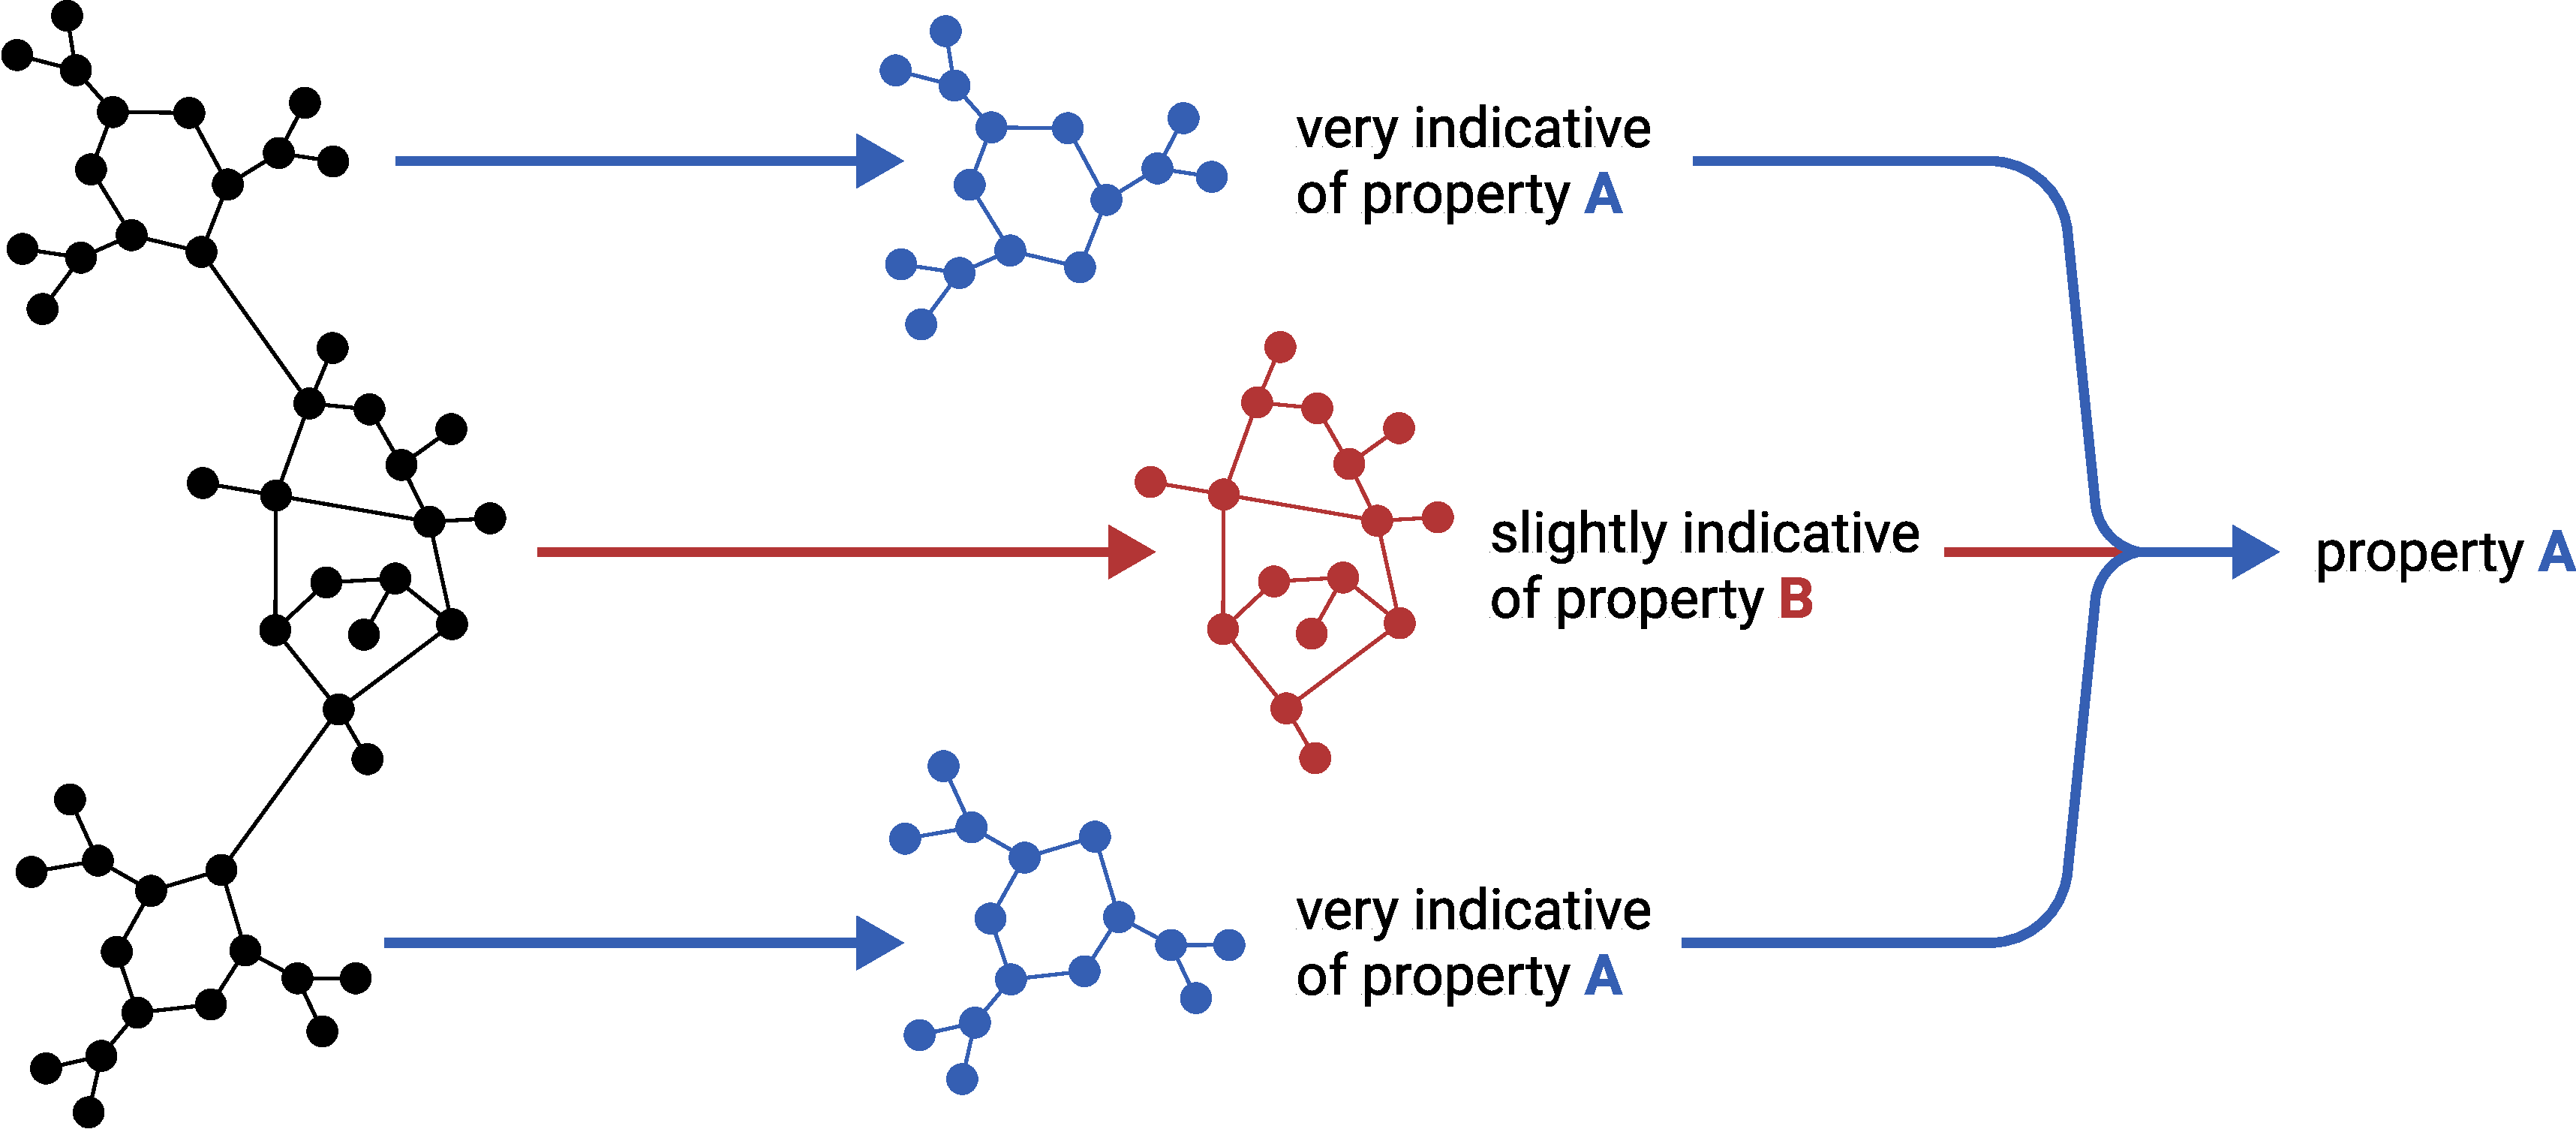
\includegraphics[width=0.8\linewidth]{gfx/introduction/intuition.pdf}
	\caption{Intuition for how \ac{lta} could describe some graph property, e.g.\ the toxicity of a molecule, via a set of local constituent predictions.}\label{fig:intro:intuition}
\end{figure}

\section{Research Questions}%
\label{sec:intro:questions}

Based on the idea of extending \ac{lta} to graphs, we state the following three research questions which will be answered in this thesis:
\begin{enumerate}[label=\textbf{\arabic*.}]
	\item \textbf{Formalization of \ac{lta}:}
		The previous work on \ac{lta} provides only a narrow definition of \ac{lta} for unstructured multiset inputs.
		The question what its essential characteristics are, on a more general level, has not yet been considered.
		Therefore we will provide the terminology and definitions to formally capture what constitutes an \ac{lta} method as opposed to a non-\ac{lta} method.
	\item \textbf{An \ac{lta} interpretation of existing \ac{gcr} methods:}
		Using the generalized \ac{lta} formalization, a selection of state-of-the-art \ac{gcr} approaches will be checked for their compatibility with \ac{lta}.
		By doing so, we answer the question whether and how existing \ac{gcr} methods are able to produce predictions which are explainable by local constituent predictions.
	\item \textbf{Definition of a novel \acs{lta}-inspired \ac{gcr} method:}
		As a follow-up question to the previous one, we ask to which extent the existing \ac{gcr} methods are explainable and what their specific shortcomings are.
		Based on those shortcomings we will propose a novel \acs{lta}-inspired approach to overcome them.
\end{enumerate}

\section{Structure}%
\label{sec:intro:structure}

\paragraph{\Cref{sec:related}: \nameref{sec:related}}
In order to answer our three research questions, we begin by with on overview of the previous work regarding \ac{lta} as well as \ac{gcr}.
We begin with a brief description of \ac{lta}.
Then the theoretical foundations of the existing \ac{gcr} approaches are introduced;
one particularly important concept there will be the so-called \acl*{wl} coloring.
Based on the theoretical foundations, we conclude the chapter by describing common graph embedding and \acl{gnn} methods.

\paragraph{\Cref{sec:ltag}: \nameref{sec:ltag}}
In this chapter we answer the first two of our research questions.
In the first step a formal definition of \ac{lta} is provided, which answers the question of what constitutes an \ac{lta} method.
This definition is then used to analyze all \ac{gcr} approaches described in \cref{sec:related} for their compatibility with \ac{lta}.

\paragraph{\Cref{sec:ltd}: \nameref{sec:ltd}}
Based on the \ac{lta} perspective on \ac{gcr} provided in \cref{sec:ltag}, we find that the existing approaches are all limited by their underlying solution to the so-called \ac*{ltd} problem.
To overcome this limitation, and thereby answer our third research question, we propose the general idea of edge-filtered graph convolutions.
To realize this general idea in a specific method, we then proceed by proposing a novel type of \ac*{gcnn}, the so-called \textit{2-\acs*{wl}-\acs{gnn}}, which can serve as the foundation for an edge-filtering-based solution to the \acs*{ltd} problem.
Apart from its uses in the context of \ac{lta}/\acs*{ltd}, we show that 2-\acs*{wl}-\acsp{gnn} have additional theoretical advantages over existing approaches;
this makes them interesting even from a non-\acs{lta} perspective.

\paragraph{\Cref{sec:eval}: \nameref{sec:eval}}
In this chapter we empirically evaluate how \ac{gcr} approaches that are compatible with our definition of \ac{lta} perform compared to non-\acs{lta} \ac{gcr} approaches.
Additionally, we compare the proposed 2-\acs*{wl}-\acs{gnn} with other state-of-the-art \acp{gnn} to verify whether its theoretical advantages over previous approaches can be observed in practice.

\paragraph{\Cref{sec:conclusion}: \nameref{sec:conclusion}}
Finally, the results of this thesis are summarized and a brief outline of promising directions for future research is given.
